%\addbibresource{/home/jorgsk/phdproject/bibtex/jorgsk.bib}
The aim for this doctoral work was to use computational tools in combination
with empirical experiments to study regulation of gene expression due to
variation in deoxynucleic acid (DNA) sequences. This aim has been met by using
calculations of free energy changes for base pairing of ribonucleic acid (RNA)
and DNA molecules to study the mechanisms of transcription initiation and
translation initiation, as well as using DNA-pattern recognition to identify
polyadenylation sites at the 3\ppp end of human messenger RNA (mRNA). The work
on transcription initiation has further been complemented by a kinetic study.
The unifying theme in this thesis work is the effect of sequence variation in
DNA and RNA leads on different aspects of gene expression.

RNA and DNA molecules are polymers of nucleotides denoted by G, A, C, and T (U
instead of T for RNA). Due to their polymer nature, RNA and DNA are also called
nucleotide chains. It is today introductory text book material that these
nucleotide chains can anneal together by base pairing to form complementary
double stranded DNA and RNA, as well as RNA-DNA hybrids. Now taken for
granted, the self-complementarity of RNA and DNA was once a tremendous
discovery and remains the very basis for life itself: the sole reason why the
genetic material can be replicated and expressed is because the
self-complementarity of double stranded nucleotides. This feature enables the
replication of DNA, the synthesis of RNA (transcription), and the synthesis of
protein (translation).

The role of double stranded DNA in DNA replication is well expressed in the
famous quote from the study by Watson and Crick \cite{watson_molecular_1953} on
the discovery of the structure of double stranded DNA: "(...) the specific
pairing we have postulated immediately suggests a possible copying mechanism
for the genetic material". In other words, the DNA helix consists of two
complementary molecules, and this complementarity enables the accurate
base-to-base replication of the genetic material.

In transcription, base pairing plays an important role through the ~9-10
nucleotide hybrid of nascent RNA and template DNA within RNA polymerase during
RNA synthesis \cite{vassylyev_structural_2007}. After incorporation, each new
RNA nucleotide becomes part of both the growing RNA chain and the RNA-DNA
hybrid that anchors the RNA to DNA. The RNA-DNA hybrid ensures that template
DNA and nascent RNA are kept together in the RNA polymerase active site; the
hybrid is therefore essential for the accurate base-by-base replication of the
genetic information from DNA to RNA.

In translation, RNA-RNA base pairing plays an important part: for the amino
acid chain to grow, a nucleotide triplet codon on mRNA must bind by base
pairing to a complementary RNA anticodon on the incoming amino-acid charged
tRNA. Additionally, the catalytic component of peptide bond formation in the
ribosome consists only of RNA \cite{steitz_rna_2003}, making translation a
highly RNA-dependent process.

Other biological processes which depend on base pairing include the formation
of secondary and tertiary structures of folded RNA; micro-RNA regulation by
hybridization to full-length RNA; and the binding of the 16S RNA of the
bacterial ribosome to the Shine-Dalgarno sequence of mRNA to
initiate protein synthesis.

These naturally evolved mechanisms of interactions between RNA and DNA show how
nucleotide chain base pairing and hybridization are fundamental to cellular
life. Additionally, nucleotide chain base pairing and hybridization also
underlie many of the experimental techniques employed in molecular biology
today. One example is polymerase chain reaction (PCR), which relies on the
temperature-dependence of the melting and annealing of double stranded DNA.
Another example is gene silencing, in which small interfering RNA (siRNA) can
be constructed to base pair with coding regions of mRNA to interfere with
protein synthesis. Another example are DNA microarrays, which rely on
constructing optimal RNA probes for hybridizing with a target DNA sequence.
Yet another example is the CRISPR/Cas DNA editing technology, which relies on
a complementary RNA-DNA hybrid for precise excision of DNA fragments.

Regardless of the biological or technical function mediated by nucleotide base
pairing, the function can be greatly influenced by the strength of the base
pair bonds. In general, GC-rich sequences form stronger base pairs than
sequences that are AT-rich, mainly due to differences in the stacking of the
GC and AT nucleotides \cite{yakovchuk_base-stacking_2006}. Look-up tables for
the strength of RNA-DNA, DNA-DNA, and RNA-RNA dinucleotide pairs (in terms of
Gibbs free energy of formation, $\Delta G$) are available in the literature,
and have a long history of use in computational biology, especially in the
field of predicting RNA secondary structures \cite{mathews_prediction_2006}. 

Nucleotide chain interactions, as mentioned, play key roles in gene expression;
from transcription initiation to translation. However, although the genetic
code of more and more organisms has been accounted for, we still only have a
limited understanding of how DNA and RNA sequence affects transcription and
translation. In this thesis we have contributed to that understanding by
investigating three aspects of gene expression that are affected by the binding
strength between nucleotide chains and the binding strength between nucleotide
chains and protein: transcription initiation, translation initiation, and
post-transcriptional RNA processing.

We have studied translation initiation (Chapter \ref{chap:celB}) through
calculations of RNA secondary structures using methods that rely on RNA-RNA
base pairing to predict how secondary structures affect the binding of the
bacterial ribosome to mRNA. By experimentally translating RNA sequences with
different predicted secondary structure, this work has contributed to a greater
understanding of several protein expression systems.

In the first study of initial transcription in this thesis (Chapter
\ref{chap:initiation_paper}), we have used calculations of the binding
strengths of double stranded DNA and the RNA-DNA hybrid in an equilibrium
model of translocation to investigate the sequence dependence of productive
transcription from a promoter. This led to the discovery of an association
between the translocation of RNAP on DNA and the production of abortive RNA
during transcription initiation. Based on this finding, transcription
initiation experiments were performed which supported the computational
findings. This has resulted in new knowledge about how the sequence of the
3\ppp terminal end of the RNA affects promoter escape in bacteria.

In the second study of initial transcription (Chapter 
\ref{chap:kinetics_paper}, we have used a kinetic model of initial
transcription to study the dynamical nature of abortive cycling. To inform the
rate constant of backtracking, we used abortive probabilities found from bulk
transcription experiments. By comparing model outcome to single-molecule
experiments of abortive cycling, we found that the speed of initial
transcription was the same as what has been reported for transcription
elongation. This has contributed new knowledge to the dynamics of initial
transcription.

In a fourth study in this thesis (Chapter \ref{chap:polyA}), we used a
genome-wide approach to study the regulation of gene expression by
polyadenylation of RNA. This work involved the analysis of nucleotide
sequences; however, instead of using free energies, the focus was on analysing
poly(A) sequences from high-throughput RNA sequencing (RNA-seq) data to study
pre-RNA processing in the form of cleavage and polyadenylation. This work has
broadened the view of the thesis by investigating the regulation of gene
expression from a genome-wide perspective, as opposed to the gene-centric
approach of the two first studies.

Figure \ref{fig:thesis_visual} summarizes the different aspects of gene
expression that are investigated in this thesis. On the left in this figure are
the aspects of gene expression that have been studied, and on the right are the
main computational methods that have been used to study them.

When studying the different aspects of gene expression we have employed two
different research approaches: for the studies with free energy and secondary
structure, a traditional gene-centric, single-molecule approach has been used;
while for the study of 3\ppp cleavage and polyadenylation a top-down,
genome-wide approach has been taken. The utilization of these two different
approaches, which can also be referred to as hypothesis-driven and data-driven,
is interesting in its own right and will make up part of the final discussion
at the end of the thesis.

\begin{figure}[htb]
	\begin{center}
		\includegraphics[scale=0.6]{illustrations/thesis_visual_abstract_portrait.pdf}
	\end{center}
	\caption{}
	\label{fig:thesis_visual}
\end{figure}
